\begin{quote}
    \textit{``What about the bifurcation sphere?'' ``It will be the throat of an Einstein-Rosen bridge. Those of you who watched Thor\ldots this will be familiar.'' --a student and Jorge Santos}
\end{quote}

Last time, we tried to extend the Schwarzschild spacetime. Our first attempt took us inside the black hole with the Eddington-Finkelstein coordinates, and we then defined the Kruskal extension by a clever rescaling of the EF coordinates. Defining Kruskal coordinates $U$ and $V$, we observe that
\begin{equation}\label{kruskaluv}
    UV=-e^{\frac{+r}{2M}}\paren{
        \frac{r}{2M}-1
        }, \quad
    \frac{V}{U}=-e^{t/2M}.
\end{equation}
Note that $U<0$ and $V>0$ for $r> 2M$ in Schwarzschild coordinates. But here's another surprise-- if we switch the signs of both $U$ \emph{and} $V$, we can still sensibly define $r(U,V)$ for $U> 0, V < 0$ via \ref{kruskaluv}.

This is an entirely new region of spacetime, which is isometric to our black hole exterior region with one notable caveat-- time runs backwards. Notice that at the event horizon, $r=2M\implies UV=0$, so either $U=0$ or $V=0$. These lines intersect at $U=V=0$, and note that at $r=0,$ we have $UV=+1$.

\begin{figure}
    \centering
    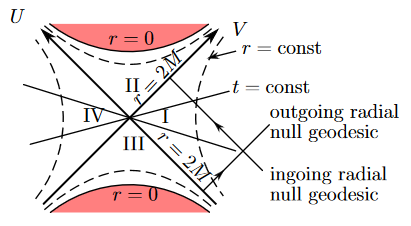
\includegraphics[width=0.5\textwidth]{2019/01/20190128_reall_kruskaldiagram.png}
    \caption{The Kruskal diagram for the Schwarzschild spacetime. There are four regions of interest: I, the original exterior; II, the black hole; III, the white hole; and IV, the mirror exterior region. (I'm not sure if there's a standard name for this.)
    }
    \label{fig:reall_kruskaldiagram}
\end{figure}
%What about the bifurcation sphere? It will be the throat of an Einstein-Rosen bridge. Those of you who watched Thor... this will be familiar.

%This if you like is part of the interior of the star. ...I just destroyed my beautiful diagram.

If we're interested in AdS/CFT, we should take all four regions seriously. However, if we're interested in astrophysical black holes, then most of the diagram is really the interior of the star as it proceeds to collapse along a geodesic.

Now recall that we have a Killing vector%
    \footnote{By the chain rule, $\P{}{t}=\P{V}{t} \P{}{V} +\P{U}{t} \P{}{U}$. Now 
    \begin{equation*}
        \P{V}{t}=\P{}{t} e^{v/4M}= \P{v}{t} \frac{1}{4M} V = \frac{1}{4M}V
    \end{equation*}
    and 
    \begin{equation*}
        \P{U}{t}=\P{}{t} (-e^{-u/4M}) = \paren{-\P{u}{t}} \frac{1}{4M}U =-\frac{1}{4M} U,
    \end{equation*} so adding it all up we have $\P{}{t} = \frac{1}{4M} \paren{ V\P{}{V} -U\P{}{U}}$.}
\begin{equation}
    K=\P{}{t}=\frac{1}{4M}\paren{V \P{}{V} -U \P{}{U}}.
\end{equation}
What happens at the point $U=V=0$?

\subsection*{The Einstein-Rosen bridge} Let us make the following coordinate transformation. Define the coordinate $\rho$ by
\begin{equation}
     r=\rho+ M +\frac{M^2}{4\rho}
\end{equation}
so that as $\rho\to +\infty, r\to + \infty$. Naturally this is quadratic(ish) in $\rho$ so we'll get two solutions for each value of $r$. We choose $\rho > M/2$ in region I, the exterior region, and $0< \rho < M/2$ in region IV. Then our metric becomes%
    \footnote{This is a bit quick-- see the end of this lecture's notes for the details.}
\begin{equation}\label{einsteinrosenmetric}
    ds^2 = -\bkt{\frac{1-\frac{M}{2\rho}}{1+\frac{M}{2\rho}}}^2 dt^2 +\paren{1+\frac{M}{2\rho}}^4\underbrace{(d\rho^2 +\rho^2 d\Omega_2^2)}_{\RR^3}
\end{equation}
So we've put the metric in a form where the spatial part looks like $\RR^3$ up to a scaling factor. It's an exercise to check that the transformation $\rho \to M^2/4\rho$ leaves this metric unchanged.

Now what does a surface of constant $t$ look like?
\begin{equation}
    ds^2_{\Sigma_t}=\paren{1+\frac{M}{2\rho}}^4\underbrace{(d\rho^2 +\rho^2 d\Omega_2^2)}_{\RR^3},
\end{equation}
As $\rho\to +\infty$, we get one asymptotically flat region, and as $\rho\to 0$ we get another asymptotically flat region.
Connecting them we get a wormhole where there is an $S^2$ at $\rho=M/2$ with some minimum (nonzero) radius.%
    \footnote{We know it's asymptotically flat as $\rho\to 0$ by the $\rho \to M^2/4\rho$ symmetry, and the value of $\rho$ that's unchanged by $\rho\to M^2/4\rho$ is $\rho=M/2$. If we were being pretentious, we might say that there's a duality between the $\rho\to 0$ and $\rho\to \infty$ regions, and $\rho=M/2$ is the self-dual point. Fixing $\rho= M/2$, we get $ds^2 = 4M^2 d\Omega_2^2$, i.e. a round 2-sphere metric with radius $2M$.}

Now, note that from our Kruskal diagram, this wormhole is non-traversable. In order to get to region IV, we must enter the black hole region. And once we're in the black hole region (region II), we are bound to hit the singularity. Tough luck.

\subsection*{Extendability and singularities}
\begin{defn}
A spacetime $(\cM,g)$ is \term{extendible} if it is isometric to a proper subset of another spacetime $(\cM',g)$. The latter is called an \term{extension} of $(\cM,g)$.
\end{defn}
Thus the Kruskal spacetime is an extension of the Schwarzschild spacetime, and moreover it is the maximal analytic extension of Schwarzschild.

Let's talk a bit about singularities now. There are different sorts of singularities we might be interested in.
\begin{itemize}
    \item Coordinate singularities: the metric (or determinant) is not smooth in some coordinate chart. Nothing physically bad has (necessarily) happened, but we just chose bad coordinates.
    \item Curvature singularities: a curvature scalar becomes singular. These are physically significant, since we cannot define them away by a coordinate choice.
    \item Conical singularities: consider the line element
    \begin{equation}
        g=dr^2 +\lambda^2 r^2 d\phi^2,
    \end{equation}
    with $\lambda>0$. We can always make this look like $dr^2+r^2 d\tilde \phi^2$, which looks like $\RR^2$. But suppose $\lambda \neq 1$. Then the period of our new $\tilde \phi=\lambda \phi$ coordinate is not $2\pi$. If we take a ``circle'' of radius $\epsilon$, we see that $\frac{\term{circumference}}{\text{radius}}=\frac{2\pi \lambda \epsilon}{\epsilon}=2\pi \lambda$, which does not go to $2\pi$ as $\epsilon\to 0$. What results is a conical singularity at the origin.
    \item There are certain metrics such that the components of the Riemann tensor are singular in every coordinate system, which means that the tidal forces become infinite as you approach the singularity. We will see an example of this on the examples sheet.
\end{itemize}
%This looks weird. But life can be even more weird!

\begin{defn}
    A \term{curve} is a smooth map from some interval of the real line to our manifold, $\gamma:(a,b) \to \cM$, with $a,b\in \RR$.
\end{defn}
\begin{defn}
    A point $p\in \cM$ is a \term{future endpoint} of a future-directed causal curve if for any neighborhood $\mathcal{O}$ of $p$, there exists $t_0$ such that $\gamma(t) \in \mathcal{O}$ for all $t>t_0$. That is, our curve gets trapped arbitrarily close to $p$ at late times.
\end{defn}
\begin{defn}
    We say that $\gamma$ is future-inextendible if it has no future endpoints. Equivalent notions of past endpoints and past-inextendible can be defined by replacing future with past, and we say a curve is inextendible if it is future-inextendible and past-inextendible.
\end{defn}
\begin{exm}
    Let $\gamma:(-\infty,0)\to \cM$, with $\gamma(t)=(t,0,0,0)$. Clearly, this has a future endpoint at $(0,0,0,0)$. If we remove that point from the manifold, however, there is no future endpoint-- no other point on our manifold will satisfy the future endpoint condition since we can always take $\gamma$ at some time arbitrarily close to zero. So the notion of extendibility depends crucially on our choice of manifold.
\end{exm}
\begin{defn}
    A \term{geodesic} is complete if an affine parameter for the geodesic exists to $\pm \infty$. A spacetime is \term{geodesically complete} if all inextendible causal geodesics are complete. A spacetime is \term{singular} if if it is inextendible and geodesically incomplete.
\end{defn}
\begin{exm}
    The Kruskal spacetime is inextendible, and it has plenty of geodesics which hit the $r=0$ singularity and are therefore incomplete. Therefore by our definition, the Kruskal spacetime is singular.%
        \footnote{In fact, incomplete geodesics are a sufficient but not necessary condition for a spacetime to be singular. We should also in principle be concerned about accelerating observers falling off the edge of spacetime into a singularity-- cf. Hawking and Ellis, and also work by Geroch. According to Hawking and Ellis, the more appropriate notion is not geodesic completeness but a more general idea of ``b-completeness,'' completeness of general inextendible causal curves in the spacetime.}
\end{exm}

\subsection*{Non-lectured aside: algebra for Einstein-Rosen}
Actually showing that the coordinate transformation gives the metric \ref{einsteinrosenmetric} is left as an exercise in Harvey Reall's notes, so I work out the details here.

First,
\begin{align*}
    1-\frac{2M}{r} = 1-\frac{2M}{\rho+M + \frac{M^2}{4\rho}} = \frac{\rho -M + \frac{M^2}{4\rho}}{\rho + M + \frac{M^2}{4\rho}} = \frac{1-\frac{M}{\rho} + \frac{M^2}{4\rho^2}}{1+\frac{M}{\rho} + \frac{M^2}{4\rho^2}} = \bkt{\frac{1-\frac{M}{2\rho}}{1+\frac{M}{2\rho}}}^2.
\end{align*}
That takes care of the $dt^2$ coefficient. Next, notice that
\begin{equation*}
    r=\rho \paren{1+\frac{M}{2\rho}}^2,
\end{equation*}
so
\begin{align*}
    dr &= d\rho \paren{1+\frac{M}{2\rho}}^2 + \rho \paren{2 \paren{1+\frac{M}{2\rho}}\paren{-\frac{M}{2\rho^2}}d\rho}\\
    &= d\rho \paren{1+\frac{M}{2\rho}}^2 +  \paren{1+\frac{M}{2\rho}}\paren{-\frac{M}{\rho}}d\rho\\
    &= d\rho \bkt{1+ \frac{M}{\rho} +\frac{M^2}{4\rho^2} - \frac{M}{\rho} -\frac{M^2}{2\rho^2}}\\
    &= d\rho \paren{1-\frac{M}{2\rho}}\paren{1 +\frac{M}{2\rho}}.
\end{align*}
It follows that
\begin{equation*}
    \paren{1-\frac{2M}{r}}^{-1} dr^2 = \bkt{\frac{1+\frac{M}{2\rho}}{1-\frac{M}{2\rho}}}^2 \paren{1-\frac{M}{2\rho}}^2\paren{1 +\frac{M}{2\rho}}^2 d\rho^2 = \paren{1+\frac{M}{2\rho}}^4 d\rho^2
\end{equation*}
and
\begin{equation*}
    r^2 d\Omega^2 = \paren{1+\frac{M}{2\rho}}^4 \rho^2 d\Omega^2.
\end{equation*}